%%%%%%%%%%%%%%%%%%%%%%% file template.tex %%%%%%%%%%%%%%%%%%%%%%%%%
%
% This is a general template file for the LaTeX package SVJour3
% for Springer journals.          Springer Heidelberg 2010/09/16
%
% Copy it to a new file with a new name and use it as the basis
% for your article. Delete % signs as needed.
%
% This template includes a few options for different layouts and
% content for various journals. Please consult a previous issue of
% your journal as needed.
%
%%%%%%%%%%%%%%%%%%%%%%%%%%%%%%%%%%%%%%%%%%%%%%%%%%%%%%%%%%%%%%%%%%%
%
% First comes an example EPS file -- just ignore it and
% proceed on the \documentclass line
% your LaTeX will extract the file if required
\begin{filecontents*}{example.eps}
%!PS-Adobe-3.0 EPSF-3.0
%%BoundingBox: 19 19 221 221
%%CreationDate: Mon Sep 29 1997
%%Creator: programmed by hand (JK)
%%EndComments
gsave
newpath
  20 20 moveto
  20 220 lineto
  220 220 lineto
  220 20 lineto
closepath
2 setlinewidth
gsave
  .4 setgray fill
grestore
stroke
grestore
\end{filecontents*}
%
\RequirePackage{fix-cm}
%
%\documentclass{svjour3}                     % onecolumn (standard format)
%\documentclass[smallcondensed]{svjour3}     % onecolumn (ditto)
\documentclass[smallextended]{svjour3}       % onecolumn (second format)
%\documentclass[twocolumn]{svjour3}          % twocolumn
%
\smartqed  % flush right qed marks, e.g. at end of proof
%
\usepackage{graphicx}
%
% \usepackage{mathptmx}      % use Times fonts if available on your TeX system
%
% insert here the call for the packages your document requires
%\usepackage{latexsym}
\usepackage{natbib}
% etc.
%
% please place your own definitions here and don't use \def but
% \newcommand{}{}
%
% Insert the name of "your journal" with
% \journalname{myjournal}
%

\usepackage{amsmath}    

\begin{document}

\title{Excess thermodynamic and elastic properties of mineral and melt solutions: modelling and implications for phase relations and seismic velocities}
%\subtitle{Do you have a subtitle?\\ If so, write it here}

\titlerunning{Excess properties of mineral and melt solutions}        % if too long for running head

\author{R. Myhill}

%\authorrunning{Short form of author list} % if too long for running head

\institute{R. Myhill \at
              Bayerisches Geoinstitut, Universit\"{a}t Bayreuth, Universit\"{a}tsstrasse 30, 95447 Bayreuth, Germany\\
              \email{myhill.bob@gmail.com}}

\date{Received: date / Accepted: date}
% The correct dates will be entered by the editor


\maketitle

\begin{abstract}


This paper describes an extension to the subregular Margules mixing model which employs intermediate compounds to define the excess thermodynamic properties of solid solutions. Mathematical derivations are provided for excess thermodynamic properties (enthalpy, entropy, volume) and their pressure and temperature derivatives (bulk modulus, thermal expansion etc.). Heuristics are suggested for intermediate compounds where individual thermodynamic properties are poorly constrained.

Examples of pyroxene, garnet and melt solutions are presented, which show that accurate modelling of phase relations and seismic velocities requires absolute excess volumes to decrease as a function of pressure. The formulation proposed here allows for a wealth of experimental data to be incorporated into solution models, and is expected to be important for geochemical and geophysical models of the Earth and other planetary bodies.

\keywords{high pressure \and excess properties \and solution model \and solid \and melt \and elasticity}
\end{abstract}



\section{Introduction}
Thermodynamic models of solid and liquid solutions are increasingly used to calculate phase relations and seismic properties over large pressure and temperature ranges. Research into mantle phase relations, subduction and differentiation of the early Earth frequently involves calculations spanning thousands of Kelvin and tens of gigapascals. Over such huge ranges, excess entropy and volume are unlikely to remain constant with respect to pressure and temperature. For example, absolute excess volumes usually decrease with increasing pressure. The implication is that to provide a good estimate of phase relations and seismic velocities, solution models must be flexible enough to accommodate changes in elastic and thermodynamic derivatives, such as the bulk modulus.

The majority of solution models take a form where excess Gibbs free energies (relative to ideal solutions) are either constant as a function of temperature and pressure, or are linear, such that interaction energies between phases $W_{ij}^{\mathcal{G}}$ take the form
\begin{equation}
  W_{ij}^{\mathcal{G}} = W_{ij}^{\mathcal{E}} + W_{ij}^{\mathcal{V}}P - W_{ij}^{\mathcal{S}}T
  \label{eqn:trad_form}
\end{equation}
The entropic $\mathcal{S}$ and volumetric $\mathcal{V}$ terms are assumed to remain constant with temperature and pressure. Indeed, in the absence of calorimetric data, it is often assumed that $W_{ij}^{\mathcal{S}} = 0$. Over small pressure and temperature ranges, a linear approximation is usually satisfactory for free energy calculations (for example, to calculate the width of a solvus or equilibrium with other phases). However, thermodynamic models are now being extended over much larger pressure and temperature ranges \citep{SLB2011, HP2011, HHPH2013, DKS2013}, where such approximations may not be satisfactory.

Thermoelastic models are also increasingly being used to interpret seismic data in terms of the temperature and composition of the deep Earth. Studies have focussed on Earth's mantle \citep[e.g.][]{DGDSBR2012, MCDRT2012, DCT2012} and core \citep[e.g.][]{SGGFMM2000,SFGMM2004}, and with the successful deployment of seismometers may soon extend to Mars \citep{GLZR2014}. Again, the bulk modulus imposed by the constant excess volume approximation may be a significant and unnecessary contributor to error in these studies, especially for metallic liquids, where excess volumes at low pressures are often very large. 

This paper first discusses some observations of excess properties in solid solutions, and the physical origins of these causes. Useful rules-of-thumb are provided to provide the reader with predictions of excess propetries were only limited information is available. An adaptation of the subregular Margules mixing model is then presented, using intermediate compounds to describe the excess properties of the solid solution. This formulation is used to model the thermodynamics of three solid solutions from the literature. 


\section{Observations and models of excess properties} 
\subsection{Observations of excess properties and their causes}

Solutions of materials which exchange ions with similar radii, charge and field strength tend to exhibit near-ideal mixing. In the geological sciences, we observe this behaviour for Fe$^{2+}$-Mg$^{2+}$ exchange, for example in the solid solutions fayalite-forsterite, ferrosilite-enstatite and almandine-pyrope. These solutions exhibit negligible excess volumes and entropies and excess energies of only a few kilojoules per mole (on a one-site basis). In contrast, exchange involving very different species is commonly associated with large excess properties. One such example is Mg$^{2+}$-Ca$^{2+}$, where the large ionic radius of Ca leads to excess energies in the tens of kilojoules (for example, in pyrope-grossular or enstatite-orthodiopside). 

In structural terms, the properties of solid solutions are influenced by differences in bond character and structural flexibility between the endmembers and chemical interactions between the endmembers within the solution. Dealing first with the volumetric properties, a large mismatch in the volumes of sites involved in ion exchange between endmembers will tend to encourage positive excess volumes. For example, the ionic radii of 8-coordinated Mg$^{2+}$ and Ca$^{2+}$ are 0.89 \AA and 1.12 \AA \citep{Shannon1976}, which leads to a positive volume excess of 0.3-1.0 cm$^3$/mol in the pyrope-grossular solid solution. However, the correlation between site-size mismatch and excess volumes is far from clear. 6-coordinated Al$^{3+}$ - Fe$^{3+}$ exchange on the octahedral site in garnet (ionic sizes 0.535 \AA and 0.645 \AA) results in a negative excess volume in the grossular-andradite system. Closer inspection of the pyrope-grossular excess volumes reveals a small region of negative excess volume at the pyrope-rich side of the binary. This observation, coupled with similar observations in many other silicate and non-silicate systems, led \cite{NW1980} to argue that ordering generally results in asymmetric negative excesses which are concentrated toward the smaller-volume endmember. The asymmetry results from large ions being more difficult to squeeze into a small site than small ions into a large site, which is itself a consequence of the asymmetry in the potential energy of bonding between ions as a function of distance.

Despite the highly dynamic nature of liquid solutions relative to solid solutions, similar effects are observed. Weakly interacting solutions (those with small enthalpies of solution) tend to have positive excess volumes, while more strongly interacting species (ones likely to undergo complexation) typically producing negative excess volumes. An interesting observation is that excess volumes are typically correlated with excess compressibilities \citep{FM1965}, in terms of magnitude and sense of asymmetry. A likely hypothesis is that the shorter bonds formed during complexation are also less compressible. It is to be expected that positively correlated excess volume and compressibility also be a characteristic of solid solutions. 

\begin{itemize}
\item XXXX Comment on thermal expansion here... $\alpha K_T$ is linear within solutions is based on the observation of \cite{WVCCJB2005}.
\end{itemize}

Vibrational contributions to heat capacity and entropy are also likely to be affected by non-ideality \citep[e.g.][]{WC2002}. To understand this, consider the Debye model of heat capacity \citep{Debye1912}, which successfully predicts the low temperature heat capacities of many minerals. This model treats lattice vibrations as phonons in a box, with the minimum phonon wavelength controlled by the atomic spacing \citep{AM1976, Grimvall1999}. Thermal energy is calculated from the phonon energy integrated over all the phonons in a lattice


\begin{eqnarray}
E = \sum_{m=1}^3 \int_0^{\infty} \left<E \right> g_m(\omega)\, d\omega, \\
\left<E \right> = \hbar \omega \left<n \right>_{BE} = \frac{\hbar \omega}{\exp{\frac{\hbar \omega}{k_B T}} - 1}, \\
g(\omega) = \left\{ \begin{aligned}
    &\frac{3 N \omega^2}{\omega_D^3}, && \text{if}\ \omega \leq \omega_D\\
    &0, && \text{otherwise}
  \end{aligned}  \right. ,\\
\omega_D^3 \stackrel{\mathrm{def}}{=}\ {6 \pi^2 c_D^3 N \over V},\\
{3 \over c_D^3 } \stackrel{\mathrm{def}}{=}\ \left< \sum_{\lambda=1}^{3} {1 \over c_{\lambda}^3 }\right>
\end{eqnarray} 
\noindent where $\hbar$ and $k_B$ are the reduced Planck and Boltzmann constants, and $\left<n \right>_{BE}$ is the number of phonons with energy $\hbar \omega$ given by the Bose-Einstein relation. $g_m$ is the density of states for each phonon mode. Each phonon has three modes, or polarization states (two transverse and one longitudinal) which have identical densities of states. The Debye sound velocity $c_D$ is the directional average of the sound velocities $c_{\lambda}$ \citep{Grimvall1999}.

The resulting thermal energy and heat capacity are
\begin{eqnarray}
\frac{E}{Nk_B} = 9 T \left({T\over \Theta_D}\right)^3\ \int_0^{\Theta_D/T} {\tau^3 \over \left(e^\tau-1\right)}\, d\tau\ ,\\
\frac{C_V}{Nk_B} = 9 \left({T\over \Theta_D}\right)^3\int_0^{\Theta_D/T} {\tau^4 e^\tau\over\left(e^\tau-1\right)^2}\, d\tau\ ,\\
\Theta \stackrel{\mathrm{def}}{=}\  {\hbar c_D \over k_B} \left( {6 \pi^2 N \over V} \right)^{1\over3}
\end{eqnarray}
\noindent $\Theta$ is the Debye temperature, which is roughly equal to the temperature where all modes are excited, and is a useful measure of the hardness of the lattice. At a given temperature, softening of materials (decreasing $\Theta$) will result in higher vibrational heat capacities (Figure \ref{fig:debye_excesses}). As $T \rightarrow \infty$, $\Delta S \rightarrow 3Nk_B\ln (\Theta_{1} / \Theta_{2})$. This additionally gives us the variation of $\Theta$ across an ideal solution at high temperature; if $x$ is the proportion of endmember $A$, then $\Theta = \Theta_A^x \Theta_B^{1-x}$.



\begin{figure}[ht!]
  \centering
  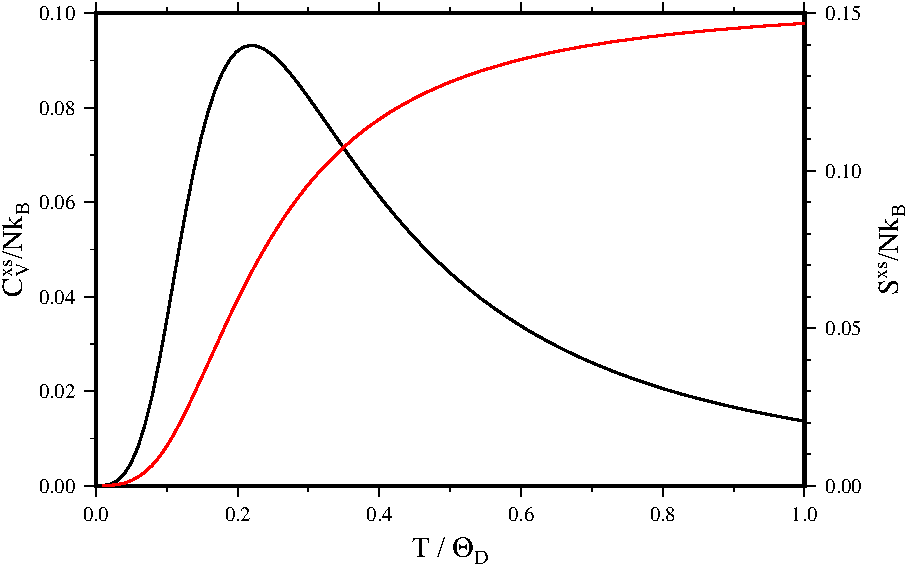
\includegraphics[width=0.8\textwidth]{figures/debye_excesses}
  \caption{Excess thermal properties as a function of temperature normalised to the Debye temperature, plotted for a reduction of 5\% in the Debye temperature.}
  \label{fig:debye_excesses}
\end{figure}

XXXX Use\cite{BD2013} for Na$_{0.2}$K$_{0.8}$Cl ($\Theta = 288^{0.2} 235^{0.8} = 244.76$ K)

Debye temperatures for geological materials are typically 600--1000 K, and so for temperatures over zeolite facies, the Debye model predicts that the vibrational contribution to excess entropy will be almost constant. Although the Debye model overestimates the density of states at high frequency, models designed to capture the high frequency behaviour (like the Einstein model) produce very similar curves. 

The preceding discussion can be summarised by the following general rules:
\begin{itemize}
\item Endmember size mismatch generally results in positive excess volume, compressibility, entropy
\item Ordering/complexation reduces the excess volume, entropy, energy and compressibility. The excess properties in both solids and liquids may become negative with sufficiently strong interactions.
\item The effects of ordering on excess properties are asymmetric with composition when there is a large mismatch in ion size. Ordering (and reduction in excess properties) is more marked for compositions rich in the phase with the smaller ion \citep{NW1980}.
\end{itemize}

\subsection{Heuristics for excess properties}

Based on the discussion in the previous section, some heuristics can be proposed which should provide a useful approximation to unknown excess properties when (for example) $V^{xs}$ is known:
\begin{eqnarray}
K_T = K_{T\textrm{ideal}} + a\\
\alpha  = \frac{\alpha K_T}{K_{T\textrm{ideal}}}, \\
\frac{\Theta}{\Theta_{\textrm{ideal}}} = \frac{V^{1 \over 6} K_T^{1 \over 2}}{V_{\textrm{ideal}}^{1 \over 6} K_{T\textrm{ideal}}^{1 \over 2}}
\end{eqnarray}

The ideal properties are given as implied by the ideal mixing model:
\begin{eqnarray}
V_{\textrm{ideal}} = 0.5\left(V_A + V_B\right),\\
\frac{V_{\textrm{ideal}}}{K_{T\textrm{ideal}}} = 0.5 \left( \frac{V_{A}}{K_{T, A}} + \frac{V_{B}}{K_{T, B}} \right) \\
\Theta_{\textrm{ideal}} = \sqrt { \Theta_A \Theta_B }
\end{eqnarray}

At high temperatures, the excess thermal properties will approach the following values:
\begin{eqnarray}
C_V^{xs} = 0, \\
S_{vib}^{xs} = 3nR \ln \left( { \Theta_{\textrm{ideal}} \over \Theta} \right)
\end{eqnarray}

\begin{itemize}
\item XXXX Use NaCl-KCl as a test
\item XXXX Also plot up an excess volume vs excess entropy model (using the Benisek and Dachs examples as starting points?)
\end{itemize}

\begin{eqnarray}
  K'_{T} = -\frac{\partial}{\partial P} \left (\mathcal{V}\left( \frac{\partial P}{\partial \mathcal{V}} \right)_T \right) \sim \mathcal{V} \left(\sum_i \frac{X_i \mathcal{V}_i}{K'_{Ti} + 1} \right)^{-1} - 1
\end{eqnarray}

If excess volumes are zero, it is likely that they will remain zero as temperatures and pressures increase. In this case, the bulk modulus is given by Equation \ref{K_T}, with the differential term equal to zero. In contrast, non-zero excess volumes are unlikely to remain constant with pressure and temperature. I suggest that, in the absence of other data a useful heuristic is $\left( \frac{\partial \mathcal{V}}{\partial P} \right)_T^{xs} \rightarrow 0$ as $P \rightarrow \infty$.

A useful way to view the change in bulk modulus across a solid solution is to compare the excess bulk modulus to that implied by the $K_TV =$ \emph{constant} rule of thumb proposed by \cite{AA1970} to estimate the compressibility of endmembers based on their molar volumes. The heuristic we propose in this study predicts a larger excess term than that suggested by the rule of thumb, which we describe using a factor $\xi$:

\begin{equation}
  K_{T} \sim 0.5(K_{Ti} + K_{Tj}) + \xi \left(\frac{K_{Ti}\mathcal{V}_{j} + K_{Tj}\mathcal{V}_{j}}{2 \mathcal{V}} - 0.5(K_{Ti} + K_{Tj})\right)
  \label{K_T_heuristic}
\end{equation}
\noindent Typically, a value of $\sim$6 provides a useful estimate of $\xi$.


%In the absence of any solid solution data, \cite{BD2011,BD2012} propose using the following equation to estimate excess heat capacities:
%\begin{eqnarray}
%\mathcal{S}^{xs, max} = a \Delta \mathcal{V} + b n \Delta K_T, \\
%\Delta \mathcal{V} = | V_{1} - V_{2} |, \\
%\Delta K_T = \frac{V_{1} - V_{2}}{| V_{1} - V_{2} |} \left( K_{T1} - K_{T2} \right)
%\end{eqnarray}
%\noindent where $n$ is the moles of ions involved in the exchange per mole of material and a and b are constants fit to experimental data. Fits to silicates, oxides and metal solutions yield values of 2.926e5 J/K/m$^3$ and 7.20e-11 J/K/Pa/mol \citep{BD2011} or 2.505e5 J/K/m$^3$ and 2.73e-11 J/K/Pa/mol \citep{BD2012}. The hypothesis underlying such equations is similar to that in the preceding section; inflated structures lead to lower frequency lattice vibrations and therefore higher heat capacities. However, the dependence on bulk modulus depends on the assumption that different cation-anion bonds have an intrinsic bond strength, which controls the magnitude and sign of the volume excess due to ion size mismatch. At least in metallic systems, bond strength is highly dependent on chemical environment \citep{WC2000}. For this reason, a simple linear dependence on bulk modulus is unlikely to be a good predictor of excess properties, which may explain the large difference in estimates for $b$.

% Estimated vibrational entropies of disordering in metal alloys may be as great as $0.5R$ \citep{TB1989; WC2002}, and therefore comparable with fully disordered configurational entropies ($\sqrt 2 R$). An increase in excess entropy with temperature must introduce an increase in the excess enthalpy, via the relation $\partial H / \partial T = T \partial S / \partial T$.

% Studies of the properties of the NaCl-KCl solid solution are in good agreement with the observations and hypotheses presented here. Excess heat capacities are positive at low temperature, and excess vibrational entropies are therefore also positive and on the order of 2 J/K/mol in the center of the binary \citep{BD2013}. Excess volumes, compressibilities and thermal expansivities are also generally positive, although sombrero-shaped excesses are reported across the solid solution for the high pressure thermal expansivities of \citep{WVCJCB2004, WVCCJB2005}.

\subsection{The Extended Subregular Margules (ESM) model}

Thermodynamic models are increasingly being used for both equilibrium phase calculations and seismic modelling, so we require that any solution model should have the following properties:
\begin{itemize}
\item Thermodynamic properties (Gibbs free energy, enthalpy, entropy) behave in a physically reasonable way at high temperature and pressure 
\item Thermoelastic properties (especially volume, bulk modulus) also behave in a reasonable way
\item Thermodynamic activities and activity coefficients should be efficiently calculable from the model
\end{itemize}

These requirements place important restrictions on the types of model formulations which are appropriate for use under extreme conditions. In particular, the third requirement is most easily fulfilled if the non-configurational excess gibbs free energy maintains a simple mathematical form across the compositional range of the solid solution at any pressure and temperature of interest. For this reason, it is best to avoid formulations that explicitly define excess properties across the solid solution (for example, via quadratic forms for excess volume, thermal expansion, bulk modulus etc.), which may well result in complex patterns across the solid solution at high pressure. Instead, excess properties can be expressed as a function of excesses in the center of each binary, along with any asymmetries.


The subregular Margules mixing model within a binary system $A$-$B$ approximates excess Gibbs free energies at any given pressure and temperature as a cubic function of composition \citep{HW1989}:
\begin{equation}
  \mathcal{G}^{xs} = X_B (1-X_B) \left(W_{AB} X_B + W_{BA} (1-X_B) \right)
  \label{eqn:subreg}
\end{equation}

In the special case that $W_{AB} = W_{BA}$, the function is a quadratic. I can define the Gibbs interaction parameter in terms of the Gibbs free energy of a 50:50 intermediate compound ($AB$) and the endmembers $A$ and $B$:

\begin{equation}
  W^{\mathcal{G}}_{AB} = 4(\mathcal{G}_{AB} + T\mathcal{S}^{\textrm{conf}}_{AB}) - 2(\mathcal{G}_A + \mathcal{G}_B)
\end{equation}
\noindent where $\mathcal{S}^{\textrm{conf}}_{AB}$ is the configurational entropy of the intermediate compound. In the more general case that $W_{AB} \neq W_{BA}$, Equation \ref{eqn:subreg} can be thought of as two symmetric interaction parameters with contributions that depend on the composition. Two intermediate compounds ($AB$ and $BA$) are then required to describe the properties of the solution (Figure \ref{fig:schematic}).

\begin{figure}[ht!]
  \centering
  %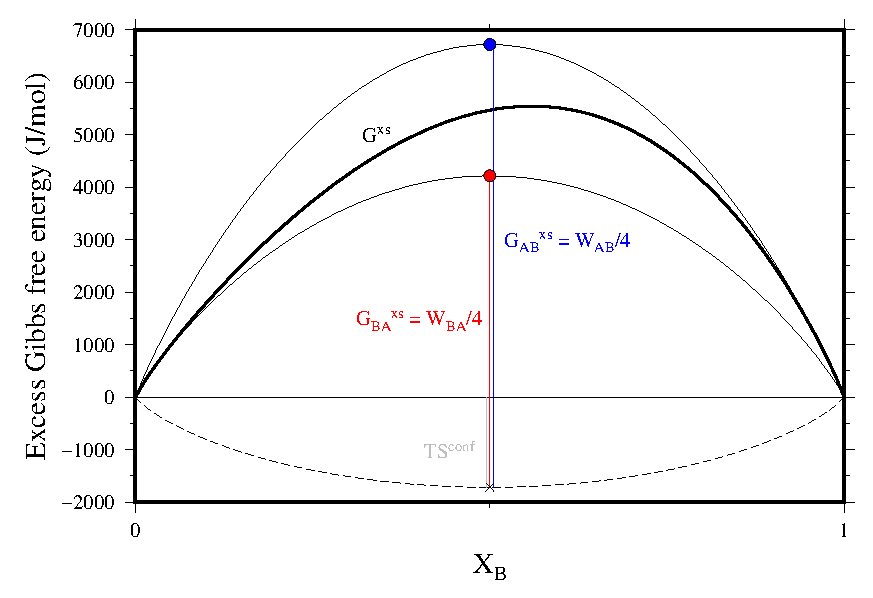
\includegraphics[width=0.8\textwidth]{figures/schematic}
  \caption{Schematic illustration of excess energies within a binary subregular solution model.}
  \label{fig:schematic}
\end{figure}


Expanding the subregular solution model beyond a binary system, the excess nonconfigurational Gibbs free energy is \citep{HW1989} 
\begin{equation}
  \mathcal{G}^{xs} = \sum_{i=1}^n \sum_{j>1}^n X_i X_j \left ( W_{ij} X_j + W_{ji} X_i + 0.5 (W_{ij} + W_{ji}) \sum_k^n (1-\delta_{ik})(1-\delta_{jk}) X_k \right)
  \label{xs}
\end{equation}

Each of the individual $W_{ij}$ terms in Equation \ref{xs} can be determined via the properties of an intermediate compound, just as described in the binary $A$-$B$ system (Equation \ref{eqn:subreg}). The properties of the solid solution with composition $\mathbf{X}$ are then defined as follows:

\begin{eqnarray}
\mathcal{G} = \sum_i X_i \mathcal{G}_i + \mathcal{G}^{xs} \\
\mathcal{H} = \sum_i X_i \mathcal{H}_i + \mathcal{H}^{xs} \\
\mathcal{S} = \sum_i X_i \mathcal{S}_i + \mathcal{S}^{xs} \\
\mathcal{V} = \sum_i X_i \mathcal{V}_i + \mathcal{V}^{xs} \\
C_P = \sum_i X_i C_P  + T \left( \frac{\partial \mathcal{S}}{\partial T} \right)_P^{xs} \\
\alpha = \frac{1}{\mathcal{V}} \left ( \sum_i X_i \alpha_i \mathcal{V}_i + \left( \frac{\partial \mathcal{V}}{\partial T} \right)_P^{xs} \right) \label{alpha} \\
K_T = \frac{\mathcal{V}}{\sum_i \frac{X_i \mathcal{V}_i }{K_{Ti}} - \left( \frac{\partial \mathcal{V}}{\partial P} \right)_T^{xs} } \label{K_T} \\
C_V = C_P - \mathcal{V} T \alpha^2 K_T \\
K_S = K_T \frac{C_P}{C_V} \\
\gamma = \frac{\alpha K_T \mathcal{V}}{C_V}   
\end{eqnarray}

With the exception of the enthalpy excess, excess terms ($\mathcal{S}^{xs}$, $\mathcal{V}^{xs}$ etc) are derived in the same way as the excess Gibbs free energy (Equation \ref{xs}), with interaction terms defined as follows:

\begin{eqnarray}
  W^{\mathcal{S}}_{ij} = 4 (\mathcal{S}_{ij} - \mathcal{S}^{\textrm{conf}}_{ij}) - 2(\mathcal{S}_i + \mathcal{S}_j) \\
  W^{\mathcal{V}}_{ij} = 4 \mathcal{V}_{ij} - 2(\mathcal{V}_i + \mathcal{V}_j) \\
  W^{\partial\mathcal{V}/\partial P}_{ij} = -4 \mathcal{V}_{ij}/K_{T{ij}} + 2(\mathcal{V}_{i}/K_{T{i}} + \mathcal{V}_{j}/K_{T{j}}) \\
  W^{\partial\mathcal{V}/\partial T}_{ij} = 4 \alpha_{ij} \mathcal{V}_{ij} - 2(\alpha_{i} \mathcal{V}_i + \alpha_{j} \mathcal{V}_j) \\
  W^{\partial\mathcal{S}/\partial T}_{ij} = \frac{4 C_{P{ij}} - 2(C_{P{i}} + C_{P{j}})}{T} 
\end{eqnarray}

Finally, excess enthalpy is defined as
\begin{equation}
 \mathcal{H}^{xs} = \mathcal{G}^{xs} + T\mathcal{S}^{xs}
\end{equation}


\section{Examples}
Now that we have described the new model and heuristics related to the construction of intermediate compounds, we turn to a few geologically relevant examples. The models in this study are all implemented in the open software \emph{burnman}, a mineral physics toolkit written in python. The software, first described in \cite{CHRU2014}, was originally designed for seismic velocity calculations. It has since been augmented with thermodynamics functionality, including a range of different models for solid solutions.


\subsection{Pyroxene}
Our first example is that of jadeite-aegirine pyroxene, an almost ideal solid solution (from a volumetric perspective). I use this model to illustrate that even when excess volumes are extremely small, excess bulk moduli are resolvable. The experimental data is that of \cite{NBLBT2006}, and the equation of state used is the Modified Tait \citep{HP2011}. The fit to the volume data is shown in Figure \ref{fig:PV_jadeite_aegirine}.

\begin{figure}[ht!]
  \centering
  %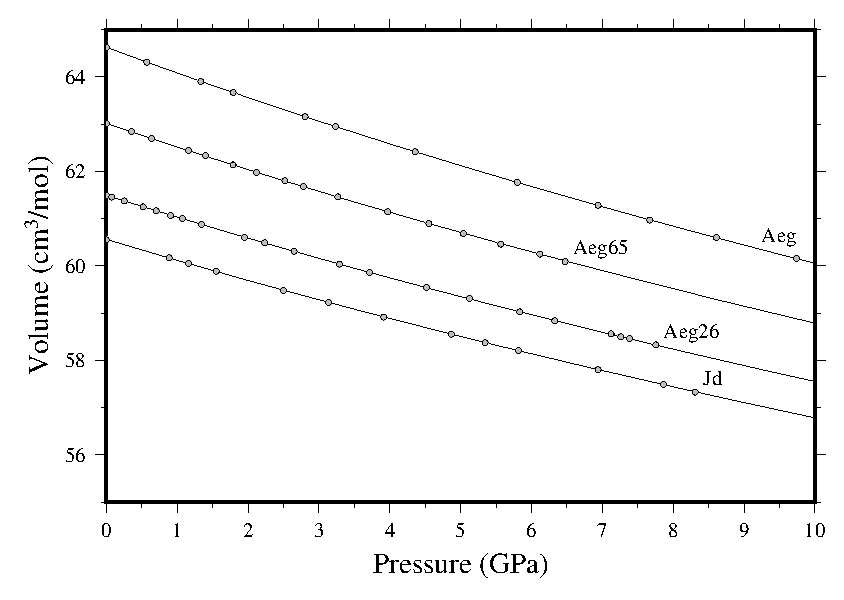
\includegraphics[width=0.8\textwidth]{figures/jadeite_aegirine_P_V}
  \caption{Pressure-volume data in the binary system jadeite-aegirine \citep{NBLBT2006}. Solid lines correspond to the volumes predicted by the model proposed in this study.}
  \label{fig:PV_jadeite_aegirine}
\end{figure}

\begin{table}[ht!]
\centering
\caption{Jadeite-Aegirine mixing parameters to fit the room temperature data of \cite{NBLBT2006}. The $K'_0$ for the intermediate compound is fixed to the value given by the heuristic proposed in the text. $K''_0 = -K'_0/K_0$.}
\label{tab:jd_aeg}
\begin{tabular}{lllll}
                   & jadeite              & aegirine             & jd$_{50}$ae$_{50}$             & ae$_{50}$jd$_{50}$             \\
$V_0$ (cm$^3$/mol) & 60.5640 $\pm$ 0.0001 & 64.6261 $\pm$ 0.0004 & 62.3641 $\pm$ 0.0005 & 62.4522 $\pm$ 0.0005 \\
$K_0$ (GPa)        & 133.5 $\pm$ 0.2      & 116.0 $\pm$ 0.2      & 124.8 $\pm$ 0.5      & 126.7 $\pm$ 0.4      \\
$K'_0$             & 4.6 [fixed]                 & 4.4 [fixed]                 & 4.4785 [heuristic]              & 4.4785  [fixed]           
\end{tabular}
\end{table}

Using the derived properties of the solid solution, we can fit the excess volume as a function of pressure (Figure \ref{fig:excess_volume_jadeite_aegirine}). The decay of excess volume as a function of pressure is in excellent agreement with the prediction that excess volumes decay to zero at extreme pressures. For the 50:50 intermediate, our excess bulk moduli and volumes indicate that $\xi \sim$ 11 (Equation \ref{K_T_heuristic}).

\begin{figure}[ht!]
  \centering
  %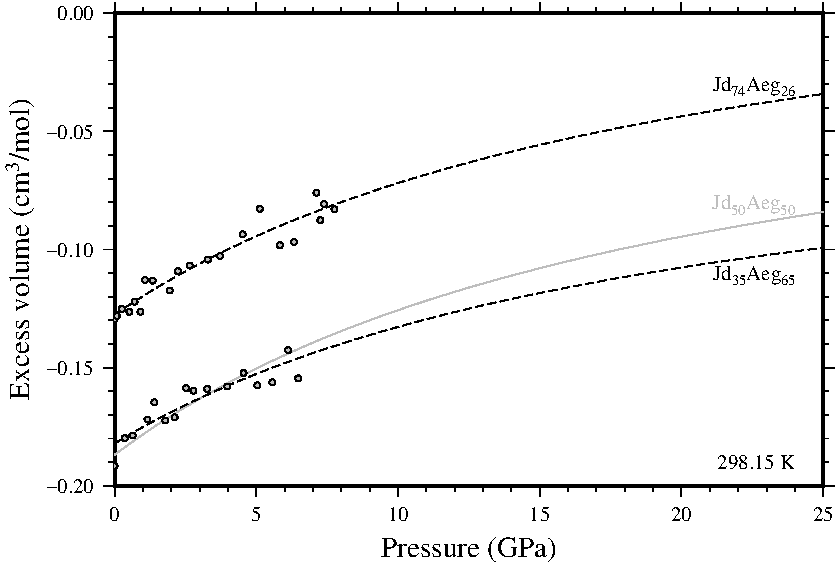
\includegraphics[width=0.8\textwidth]{figures/jadeite_aegirine_Vex}
  \caption{Excess volume for jadeite-aegirine pyroxenes \citep{NBLBT2006}. Solid lines correspond to the modelled excess volumes.}
  \label{fig:excess_volume_jadeite_aegirine}
\end{figure}

\subsection{Garnet}
Our first example dealt with a solid solution which has small excess volumes, but some phases exhibit significantly larger excesses. One example is the garnet system. Of particular interest is the pyrope-grossular join. Grossular is a major secondary component of many natural pyropic garnets. The size mismatch between the small magnesium cation and the large calcium cation on the dodecahedral site results in a large positive excess volume \citep{NCK1977, BG1997, GCT1996}. Recently, it has been suggested that the excess volumes of mixing are $\sim$1 cm$^3$/mol, 2--3 times larger than previously considered, and associated with very large negative excess bulk moduli \citep{DCW2015}. It is proposed that the differences are due to a hydrogrossular component in the crystals synthesised in piston cylinder apparatus in earlier studies, which becomes unstable at high pressures. Such a large variation in bulk modulus would have a major impact on seismic velocities and excess properties at high pressure. Since garnets remain stable to the uppermost lower mantle, a careful analysis of these effects is warranted.

Here, we create four models to describe the room temperature equations of state for the pyrope-grossular system using the pyrope and grossular endmembers from \cite{HP2011}. Two models are presented for the data of \citep{DCW2015}, to describe the reported behaviour close to the center and at the edges of the solid solution. The third model is the constant volume subregular Margules model of \cite{GCT1996}. A fourth model has the same excess volume as \cite{GCT1996}, but a negative excess bulk modulus which allows the excess volume to decay to zero at high pressures ($\xi=6$). The standard state bulk moduli are shown in Figure \ref{fig:K_T_pyrope_grossular}.


\begin{figure}[ht!]
  \centering
  %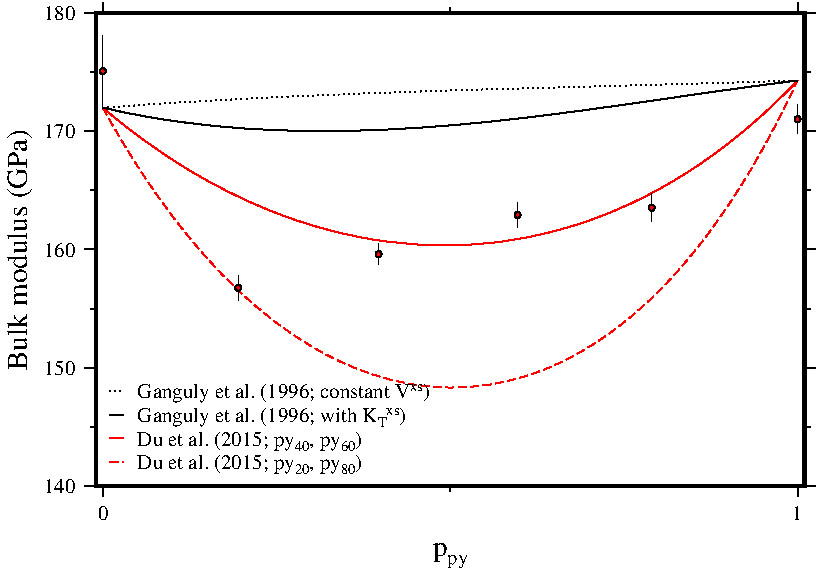
\includegraphics[width=0.8\textwidth]{figures/pyrope_grossular_K_0}
  \caption{Bulk moduli in the pyrope-grossular binary. Data points are those reported by \cite{DCW2015}. The four models correspond to those discussed in the main text.}
  \label{fig:K_T_pyrope_grossular}
\end{figure}

It is immediately obvious that the bulk moduli calculated from the \cite{DCW2015} study exhibit very large deviations from a linear trend. The symmetric curve derived from the two compounds in the middle of the binary yields $\xi=10$, a value which is not unreasonable, and results in a change in sign of the volume excess at 20--25 GPa. In contrast, the trend derived from the compounds with 20\% and 80\% pyrope content yields $\xi=52$. This extreme value leads to negative excess volumes at 5--6 GPa, which does not seem to be very likely. To avoid this, $K'_T$ must be increased to $>$20, which is also extremely unlikely.

The trend calculated from the terms in \cite{GCT1996} has a small positive excess bulk modulus, which is always the case where $\mathcal{V}^{xs}$ is held fixed. For the reasons outlined in the introduction, this is probably unlikely. The final model, constructed using the heuristics described in the previous section yields an excess bulk modulus on the order of 2--3 GPa.

These models are now used to illustrate the effect of different excess volume models on seismic wave velocities. P-wave, S-wave and bulk sound velocities are functions of isentropic bulk and shear moduli and density:
\begin{eqnarray}
V_P = \sqrt \frac{K_S + \frac{4}{3} G }{\rho} \\
V_S = \sqrt \frac{G}{\rho} \\
V_\Phi = \sqrt \frac{K_S}{\rho}
\end{eqnarray}
Thermodynamic solution models say nothing about shear moduli, so we restrict our discussion to the bulk sound velocity. Figure \ref{fig:bulk_sound_garnet} shows the bulk sound velocity at ambient temperature for the four solid solution models in the text. The models of \cite{DCW2015} result in large depressions of bulk sound velocity. The model constructed from the py$_{40}$ and py$_{60}$ samples results in a 4\% depression relative to the constant $\mathcal{V}^{xs}$ case throughout the upper mantle pressure range. In contrast, the model based on the excess volume model proposed in \cite{GCT1996} predicts a 1\% decrease in bulk sound speed. 

\begin{figure}[ht!]
  \centering
  %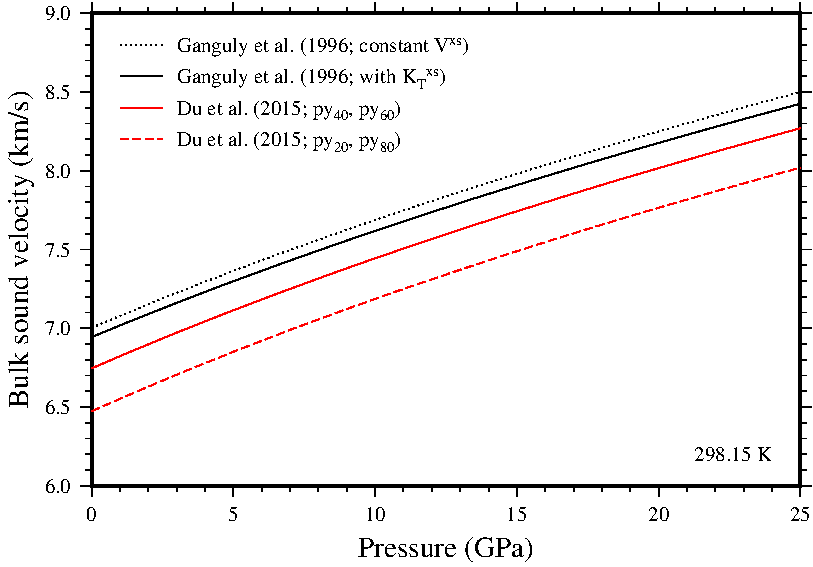
\includegraphics[width=0.8\textwidth]{figures/pyrope_grossular_bulk_sound_velocities}
  \caption{Bulk sound velocities of py$_{50}$gr$_{50}$ at room temperature according to the models described in the text and in Figure \ref{fig:K_T_pyrope_grossular}.}
  \label{fig:bulk_sound_garnet}
\end{figure}

It is not yet clear whether natural garnets have P-V-T equations of state similar to those suggested by \cite{DCW2015}, or similar to those in previous studies \citep{NCK1977, BG1997, GCT1996}. If a hydrogrossular component is indeed the cause for low excess volumes in piston cylinder-synthesised garnets, then garnets in the mantle are likely to have relatively high volume excesses and low bulk moduli. In this case, constant V$^{xs}$ models are clearly inappropriate both for calculations of mantle phase relations and seismic velocities. Even in the case of the model derived from \cite{GCT1996}, the difference in free energy compared with the constant V$^{xs}$ model is on the order of kilojoules at the bottom of the mantle transition zone. 

The heuristics suggested here place constraints on seismic properties which are significantly more strict than typical uncertainties on bulk moduli derived from ultrasonic interferometry, Brillouin scattering or static compression. For example, along the pyrope-majorite join, excess volumes are small (0.1 cm$^3$/mol) \citep{HSSR1997}. With the assumption that excess volumes decrease to zero with increasing pressure, the excess bulk modulus is constrained to be $\sim$-0.6 GPa. In comparison, the range in bulk modulus estimates anywhere along the pyrope-majorite join is about 10 GPa \citep[see, for example][]{HDLWB2010}. So far, high pressure elasticity studies have mostly been focussed on binary joins with small excess volumes at ambient pressure \citep{FXMLX2015, HC2014}. That they should exhibit small excess bulk moduli is in excellent agreement with the heuristics proposed here, but a far more rigorous test would be to investigate systems with large volume excesses.

\subsection{Metallic-ionic melt}
The thermodynamics and thermoelastics of ionic and metallic melts is fundamental to our understanding of core differentiation. During the formation of the terrestrial planets, it is thought that oligarchic growth led to a series of mixed silicate-metallic magma oceans, from which metallic melts separated before sinking as diapirs into the growing core \citep{Rubieetal2015}. Although these melts are predominantly composed of iron and nickel, several weight percent of light elements are required to explain the Earth's density deficit and low seismic velocities \citep{Poirier1994}. These light elements not only influence the melting point of the core (which directly informs us about the temperature of the inner core boundary), but also the style of crystallisation, and therefore the generation of a magnetic dynamo \citep{SSWL2007}. Since equilibration with a magma ocean governs the initial composition of the core, and seismology presents us with the most direct information on the present composition of the core, accurate thermodynamic modelling is vitally important to our understanding of the evolution and present chemical state of the Earth. It is well known that several iron-light element binaries are associated with large non-idealities \citep[e.g.][]{Frostetal2010}, so accurate modelling requires changes in excess properties in these systems to be taken into account.

Oxygen is a good example of a light element which exhibits a large degree of non-ideality. At pressures $<$25 GPa, the Fe-FeO solution exhibits significant non-ideality, with a large miscibility gap between ionic and metallic Fe-O liquids \citep{KS1995,TOT2007,Frostetal2010}. As pressure increases, this miscibility gap disappears, indicating a negative excess volume of mixing (Figure \ref{fig:Fe_O_solvus}).

\begin{figure}[ht!]
  \centering
  %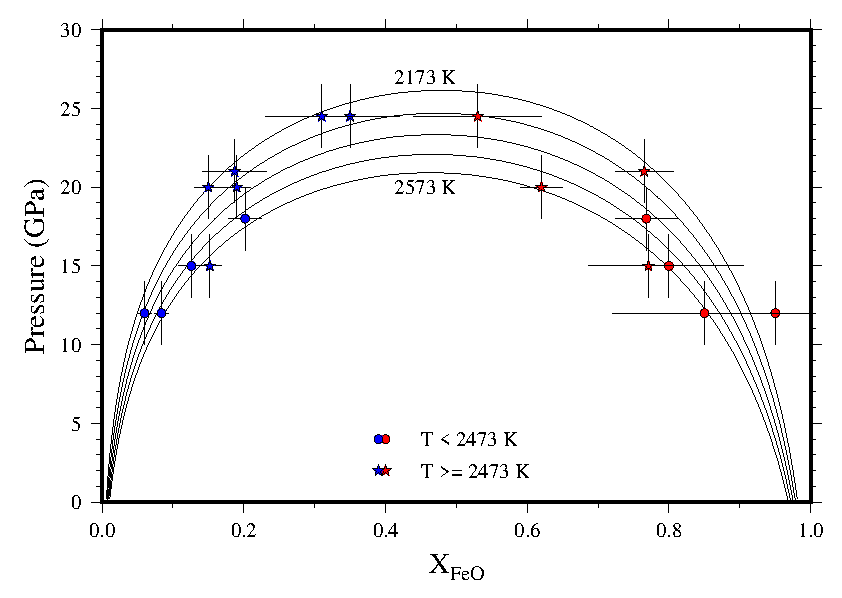
\includegraphics[width=0.8\textwidth]{figures/Fe_FeO_solvus}
  \caption{The Fe-FeO solvus as a function of pressure and temperature. Data points are taken from the studies of \cite{TOT2007} and \cite{Frostetal2010}. The model corresponds to the values proposed in Table \ref{tab:Fe_FeO}.}
  \label{fig:Fe_O_solvus}
\end{figure}

To constrain the properties of the Fe-FeO solid solution, the chemical potentials of Fe and FeO are estimated from the compositions of coexisting ionic and metallic melts at $<$25 GPa, and the pressure, temperature and compositions of eutectic liquid at $>$25 GPa \citep{SHCPW2008}. The latter constraints also require thermodynamic data for the eutectic phases (B1-structured FeO and FCC and HCP iron), which are calculated from room pressure data and constraints on the melting curves \citep{SHCPW2008, OTHOH2011, ADMLM2013, Kom2014}.  The Margules parameters estimated from this data are shown in Figure \ref{fig:Fe_O_interaction}. 

\begin{figure}[ht!]
  \centering
  %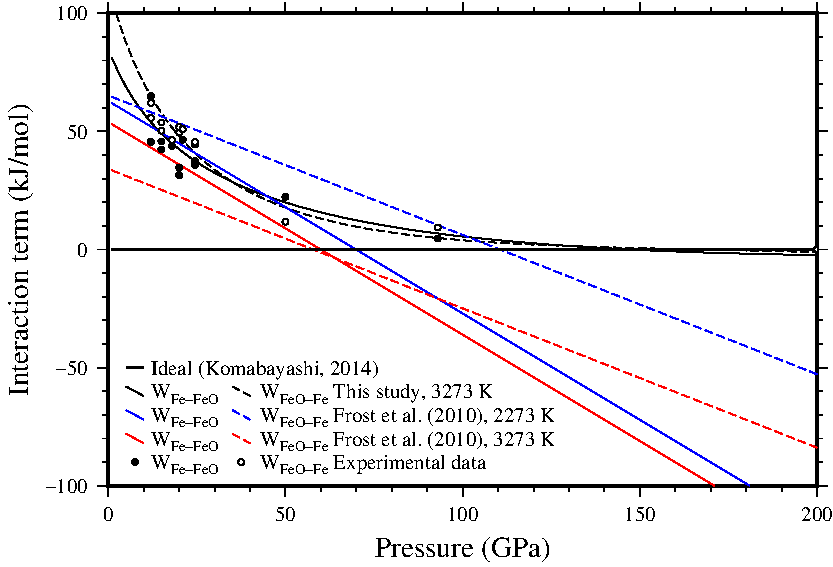
\includegraphics[width=0.8\textwidth]{figures/Fe_FeO_interaction_terms}
  \caption{Interaction terms in Fe-FeO melt as a function of pressure. Experimental data comes from solvus constraints at $<$25 GPa \citep{TOT2007,Frostetal2010}, and the composition and temperature of the eutectic at higher pressures \citep{SHCPW2008}.}
  \label{fig:Fe_O_interaction}
\end{figure}

The uncertainties on composition and temperature of the eutectic are rather large, so these data are supplemented by the requirement that excess volumes become zero at very high pressure. The parameters used to create the fits in Figures \ref{fig:Fe_O_interaction} and \ref{fig:Fe_O_melting} are given in Table \ref{tab:Fe_FeO}. It is assumed that excess entropy and thermal expansion are negligible. The majority of the $<$25 GPa data was collected within a $\sim$200 K temperature range, and is associated with similar temperature uncertainties, which introduces very large uncertainties in excess entropies. Add to that the possibility of phase separation during quench and the large uncertainty in coexisting ionic/metallic melt compositions, there is no clear evidence for the large temperature dependence proposed by \cite{Frostetal2010}, although they do slightly improve the fit to the data (mostly by increasing the pressure at which the solvus closes at high temperature).

\begin{figure}[ht!]
  \centering
  %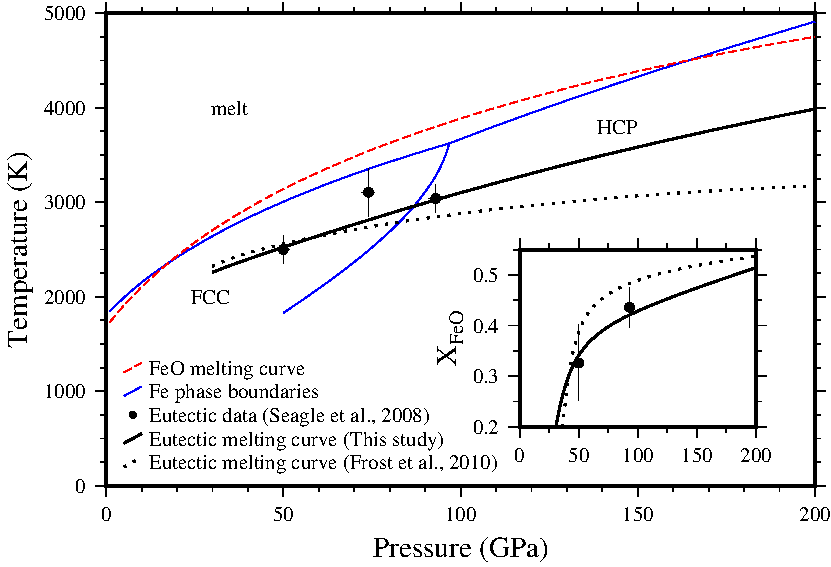
\includegraphics[width=0.8\textwidth]{figures/Fe_FeO_T_X_eutectic}
  \caption{Melting temperature in the Fe-O system as a function of pressure. Inset: eutectic composition in the Fe-O system. Data points are from \cite{SHCPW2008}. The model of \cite{Frostetal2010} employs constant volume and entropy terms derives from data obtained at $<$25 GPa, and deviates significantly from experimental constraints at pressures corresponding to the Earth's core.}
  \label{fig:Fe_O_melting}
\end{figure}

\begin{table}[ht!]
\centering
\caption{Excess Fe-FeO mixing parameters to fit the data in Figures \ref{fig:Fe_O_interaction} and \ref{fig:Fe_O_melting} at a reference temperature of 1809 K and pressure of 50 GPa.}
\label{tab:Fe_FeO}
\begin{tabular}{lll}
  Property        & Fe$_{50}$FeO$_{50}$  & FeO$_{50}$Fe$_{50}$ \\
  $H^{xs}$ (J/mol) &  5000 $\pm$ 400 & 4400 $\pm$ 400  \\
  $S^{xs}$ (J/K/mol)  & 0 [fixed] & 0 [fixed] \\
  $V^{xs}$ (cm$^3$/mol)   & -0.117 $\pm$ 0.009 &  -0.138 $\pm$ 0.009 \\
  $K^{xs}$  (GPa)  & 28 $\pm$ 5 & 45 $\pm$ 5  \\
  $K'^{xs}$   & -0.07 $\pm$ 0.12 & -0.37 $\pm$ 0.12  \\
  $a^{xs}$   & 0 [fixed] & 0 [fixed]  
\end{tabular}
\end{table}


The constant negative volume excesses in the model of \cite{Frostetal2010} produce reasonable eutectic melting temperatures up to $\sim$ 50 GPa. Beyond this point, the increasing pressure stabilisation of the solution results in large deviations from the slope of the melting curve (Figure \ref{fig:Fe_O_melting}). This effect becomes very large at inner core boundary pressures (330 GPa), where solid Fe and FeO are stable to at least $\sim$4200 K \citep{OTHOH2011}. In contrast, the melting point derived from the parameters of \cite{Frostetal2010} reaches a maximum at 3225 K and 275 GPa. The best fit excess bulk moduli in Table \ref{tab:Fe_FeO} are large, even at the reference pressure of 50 GPa. Such values will have a significant effect on seismic velocities, especially at the pressures corresponding to the cores of small planetary bodies.


\section{Discussion}
% Intro
The use of intermediate compounds to describe excess properties within the framework of simple solution models lends the flexibility required to create single thermoelastodynamic models covering very large \emph{P-T} ranges. In this study, the high pressure properties of pyroxenes, garnets and melts are used to illustrate the development of such models, and their ability to accurately reproduce observed variations in pressure, temperature or compositional derivatives of the Gibbs free energy, such as bulk modulus and chemical potentials. Without these, it would be impossible to accurately model phase relations at extreme conditions, or seismic velocities.

This study does not discuss the behaviour of the shear modulus across solid solutions. Thermodynamic databases are now starting to include shear moduli and their change with pressure and temperature \citep{SLB2011}, so constraining these changes across solid solutions should also be a key priority for experimental and ab-initio studies. Using intermediate compounds to describe the change in shear modulus across a solid solution should work well, especially in silicate systems, where excess shear moduli may be of similar magnitude to excess bulk moduli, and also decrease with increasing pressure \citep[e.g][]{LEDD2014}.

% Heuristics
The heuristics suggested in this study agree with the available data on the three example systems, but remain heuristics only. It would be particularly interesting to investigate the change in excess volumes with temperature and pressure for other systems in which excess properties are large, and interpret these in terms of crystal or melt structures. Conversely, the behaviour of systems with small excesses at room temperature and pressure should also be investigated. Current evidence suggests that small volume excesses at low pressure remain small under different conditions \citep{FXMLX2015, HC2014}, but this may not be true for all solutions.

% Other planets
In the case of ionic and metallic melts, excess volumes can be extremely large at low pressure. The large excess elastic moduli accompanying these excess volumes will have a large effect on seismic velocities, especially in the cores of relatively small bodies such as Mars or the Moon. As pressures increase, excess volumes are much reduced, which has a similarly profound effect on thermodynamic properties \citep{Frostetal2010, DKS2013}. Accurate characterisation of excess properties of melt solutions, and indeed of solutions in general, will become increasingly important for our interpretation of seismic anomalies, modelling of phase relations, and our understanding of planetary evolution. 

\begin{acknowledgements}
The author is funded by the Advanced ERC Grant awarded to the ``ACCRETE'' project (Contract number 290568). He would like to thank Dave Rubie, Dan Frost and Christopher Beyer for useful discussions.

Figures were created using the Generic Mapping Tools \citep{GMT}.
\end{acknowledgements}

\bibliographystyle{spbasic}
\bibliography{references_xs}


\end{document}

\grid
